% !TeX root = Trafficsimulation_Documentation.tex

\chapter{Software-Architektur}
\label{Software-Architektur}

In diesem Kapitel wird die Architektur in Form des Arc42-Templates sowohl grafisch als auch textuell dargestellt. 

\thispagestyle{standard}
\pagestyle{standard}

\section{Randbedingungen}
\label{Randbedingungen}

Die Verwendung der Programmiersprache C\# und die Auslagerung der Logik für geregelte Kreuzungen sind als Vorgaben für die Realisierung der Verkehrssimulation gegeben. 

Es sollen verschiedene Einstellungen zur Laufzeit geändert werden können, um die Simulation entsprechend zu strapazieren. Dazu gehören:

\begin{itemize}  
\item Anzahl der maximalen Fahrzeuge während der Simulation
\item Maximale Geschwindigkeit der Fahrzeuge
\item Die Zeit in der neue Fahrzeuge erstellt werden
\item Verhältnis zwischen PKW und LKW
\end{itemize}

Des Weiteren soll über eine vorab definierte Schnittstelle ein Austausch von Fahrzeugen innerhalb der Gruppen erfolgen können.

\section{Kontextabgrenzung}
\label{Kontextabgrenzung}

Einschränkungen im Detailgrad sowie im Umfang der Implementierung wurde keine vorgegeben. Es soll nur die Aufgabe mit den vorgegebenen Randbedingungen erfüllt werden. Wie diese umgesetzt werden, ist dem Projektteam überlassen.

\section{Lösungsstrategie}
\label{Lösungsstrategie}

Da ein Teil der Projekt Mitarbeiter bereits Erfahrungen mit Unity gemacht haben, wurde überlegt, diesen auf für die Verkehrsimulation zu verwenden. Durch die Verwendung des Unity Editors, welche als Laufzeit- und Entwicklungsumgebung für Spiele dient, wird ein Großteil bereits von der von Unity zur Verfügung gestellten "Game Engine" abgenommen. 
Da Unity eine 2D bzw. 3D Game Engine zur Verfügung stellt wurde überlegt, welche von beiden die meisten Vorteile für eine Verkehrssimulation bringt. Da jedoch der Unterschied nur in der grafischen Darstellung liegt, was bedeutet das Logik von Autos, Straße, Ampeln usw. sowohl in 2D, als auch in 3D implementiert hätte werden müssen. Da eine Simulation mit 3D Modellen ansprechender aussieht, fiel die Entscheidung auf die 3D Implementierung.

Eine weitere Lösungsstrategie ist das Aufteilen der Aufgabenbereiche. Folgende Teilbereiche für die Implementierung wurden überlegt:

\begin{itemize}  
\item Ampelsteuerung
\item Erstellung von Straßen und Kreuzungen
\item Logik und Verhalten in Fahrzeugen
\item Straßenlogik (Waypoints)
\end{itemize}

\section{Bausteinsicht}
\label{Bausteinsicht}

In diesem Abschnitt folgt die Beschreibung der Komponenten.

\begin{figure}[H]
\begin{center}
	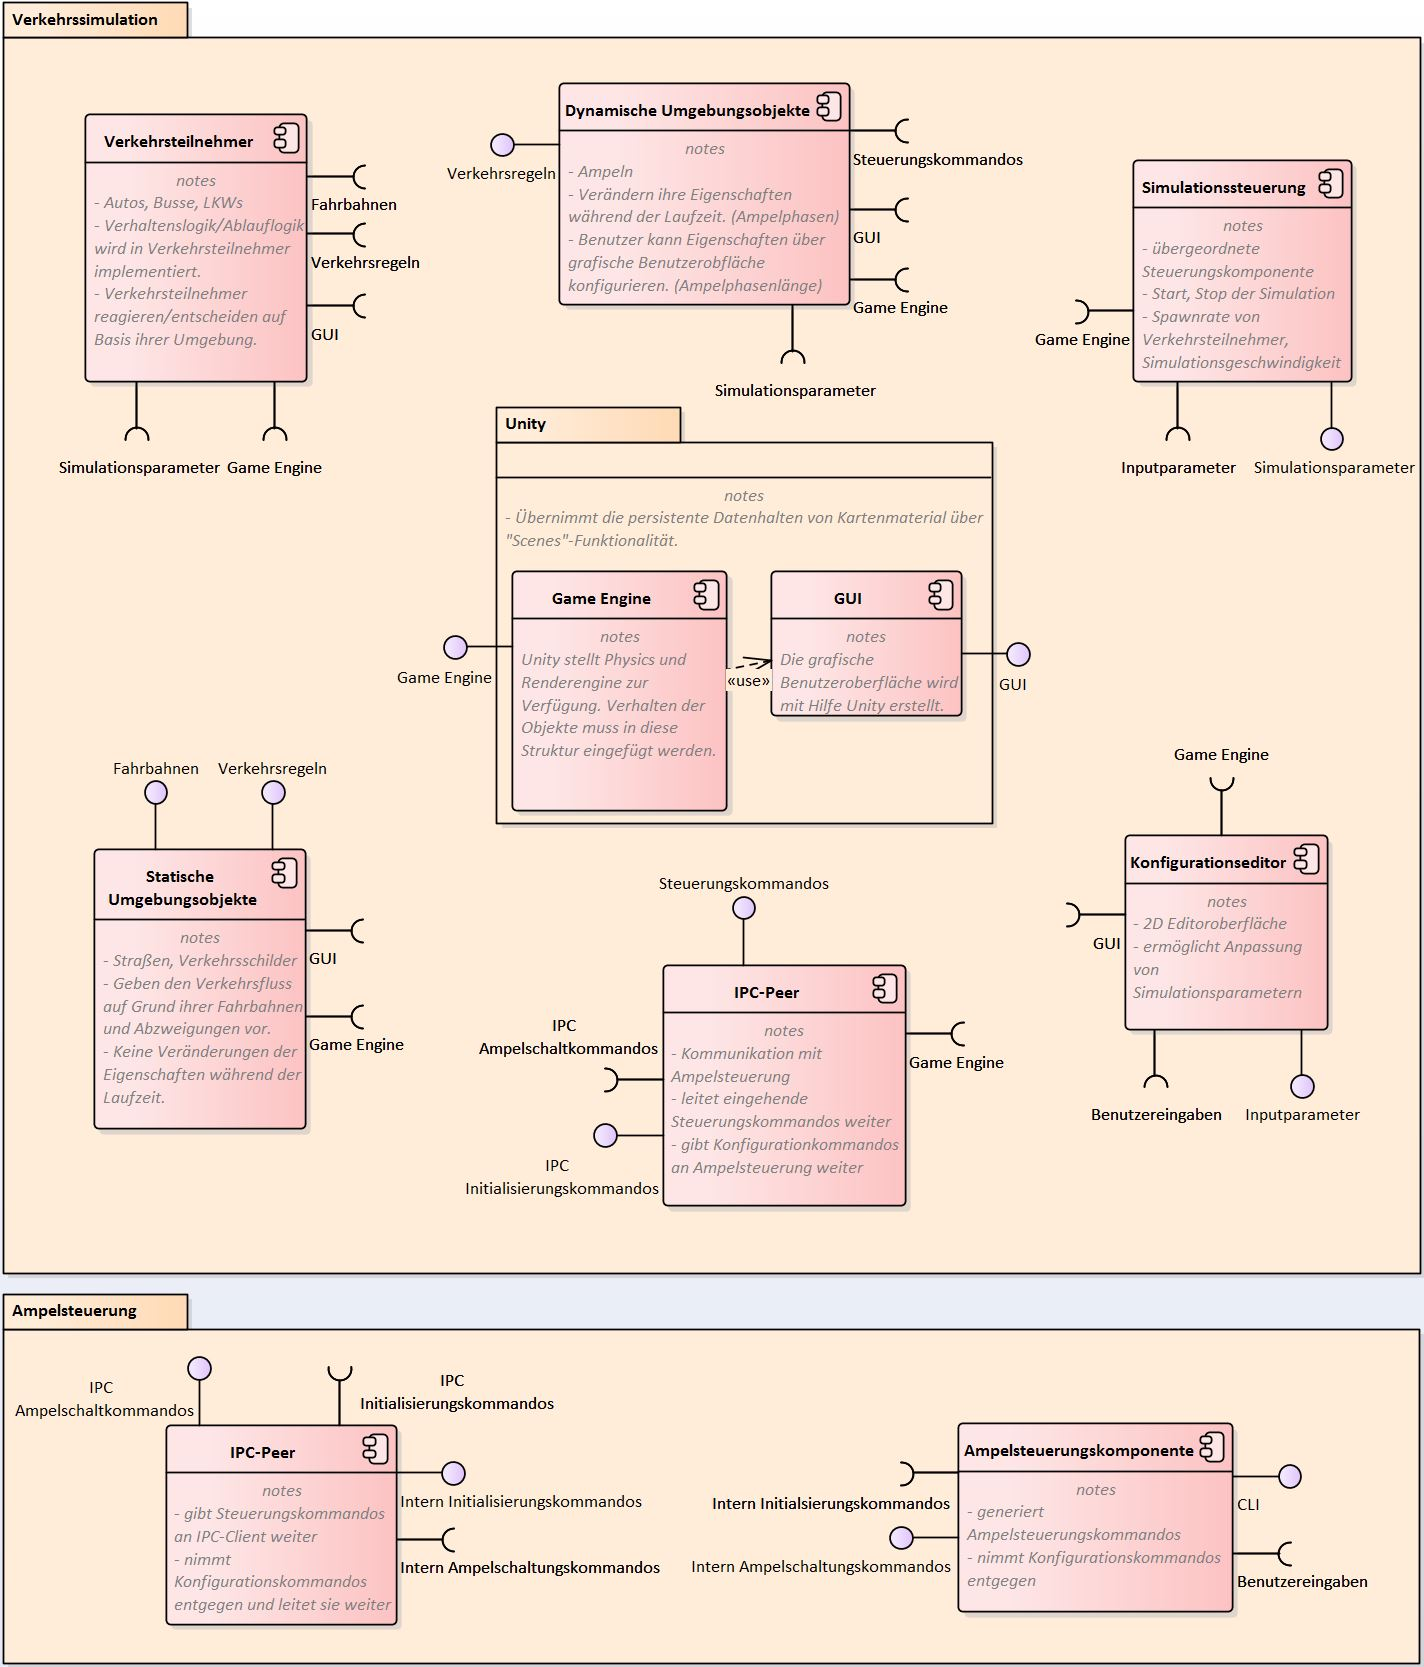
\includegraphics[scale=0.673]{BilderAllgemein/Komponentdiagram.JPG}
\end{center}
	%\includegraphics[width=\textwidth]
	%\end{center}
	% Title
	\caption{Komponenten Diagramm Verkehrssimulation}
	% Unique name: identifier for referencing
	%\label{Abbildung 2.1}
\end{figure}

\begin{flushleft}
\textbf{Verkehrssimulation und Ampelsteuerung}
\end{flushleft}
\vspace{-0.3 cm}

Sowohl Verkehrssimulation als auch Ampelsteuerung sind eigene Executables. Die Verkehrssimulation wird aus dem Unity-Projekt erzeugt und beinhaltet alle oben angegebenen Komponenten. Die Ampelsteuerung ist eine Konsolen Applikation, welche über die IPC-Komponenten mit der Verkehrssimulation kommuniziert.

\begin{flushleft}
\textbf{Verkehrsteilnehmer}
\end{flushleft}
\vspace{-0.3 cm}

Zu diesen Komponenten gehören alle sich aktiv in der Simulation bewegenden Objekte, wie Autos, Busse und LKWs. Die einzelnen Komponenten bewegen sich autonom voneinander im Straßennetz fort. Die Komponenten scannen ihre Umgebung auf Fahrbahnen, Verkehrsregeln und andere Verkehrsteilnehmer. Auf Basis dieses Scans entscheiden sie ihre nächste Aktion, wie zum Beispiel Beschleunigen, Bremsen oder Abbiegen. Verkehrsteilnehmer können sich ausschließlich auf Fahrbahnen bewegen und beachten alle Verkehrsregeln innerhalb ihres Aktionsradius. Weiters benötigen sie Simulationsparameter, die über ihre maximale Geschwindigkeit, Beschleunigung und Bremsverhalten entscheiden. Verkehrsteilnehmer treffen ihre Entscheidungen bei jedem Renderdurchlauf der Game Engine. Die Verknüpfung der Verkehrsteilnehmer mit der GUI erfolgt abstrahiert durch Unity.

\begin{flushleft}
\textbf{Dynamische Umgebungsobjekte}
\end{flushleft}
\vspace{-0.3 cm}

Dynamische Umgebungsobjekte sind Objekte, welche während der Simulationslaufzeit ihre Eigenschaften ändern, jedoch nicht ihre Position. Konkret sind dynamische Umgebungsobjekte Ampeln. Ampeln bieten den umliegenden Verkehrsteilnehmern ihren derzeitigen Status als Verkehrsregeln an, welche diese beachten müssen. Dynamische Elemente benötigen Simulationsparameter, welche ihre Schaltzeiten vorgeben. Konkret geben die Simulationsparameter die Phasenzeiten der Ampeln an. Weiters benötigen dynamische Umgebungsobjekte Steuerungskommandos um zwischen diversen Modi zu wechseln. Über Steuerungskommandos können Ampeln von automatischen Betrieb in einen inaktiven dauerhaft Gelb blinkenden Status gebracht werden. In jedem Renderzyklus der Game Engine wird auf neue Steuerungskommandos geprüft und falls nötig der vorgegebene Schaltvorgang eingeleitet. Die Verknüpfung der dynamischen Umgebungsobjekte mit der GUI erfolgt abstrahiert durch Unity.

\begin{flushleft}
\textbf{Simulationssteuerung}
\end{flushleft}
\vspace{-0.3 cm}

Die Simulationssteuerung stellt eine übergeordnete Kontrollinstanz der Simulation dar. Sie legt globale Einstellungen für Simulationskomponenten zentral fest. Die Simulationssteuerung bietet Simulationsparameter für andere Simulationskomponenten an, welche diese abrufen können. Konkrete Simulationsparameter sind Schaltzeiten für Ampeln, Höchstgeschwindigkeiten für Verkehrsteilnehmer oder Spawnraten für neue Verkehrsteilnehmer. Die Simulationssteuerung benötigt Inputparameter, welche von außen die Simulationsparameter bestimmen. Die Aktualisierung der Simulationsparameter auf Basis der Inputparameter erfolgt bei jedem Renderzyklus der Game Engine.

\begin{flushleft}
\textbf{Konfigurationseditor}
\end{flushleft}
\vspace{-0.3 cm}

Der Konfigurationseditor stellt eine zweidimensionale graphische Benutzeroberfläche dar, welche es dem Benutzer ermöglicht angebotene Inputparameter für die Simulation zu verändern. Vom Benutzer geänderte Inputparameter werden bei jedem Renderzyklus der Game Engine verarbeitet und entsprechend weiter geleitet.

\begin{flushleft}
\textbf{IPC-Peer Verkehrssimulation}
\end{flushleft}
\vspace{-0.3 cm}

Der IPC-Peer Verkehrssimulation repräsentiert eine Instanz der Inter Process Communication zwischen den Executables Verkehrssimulation und Ampelsteuerung dar. Dieser IPC-Peer gibt Initialisierungskommandos an die Ampelsteuerung weiter. Über diese Kommandos werden die benötigte Anzahl an Ampeln mit den korrekten Initialisierungsparametern angelegt. Weiters werden Ampelschaltkommandos entgegen genommen und weiter geleitet um den Modus einer Ampel zu wechseln. Ein- und ausgehende Kommandos während in jedem Renderzyklus der Game Engine bearbeitet.

\begin{flushleft}
\textbf{Statische Umgebungsobjekte}
\end{flushleft}
\vspace{-0.3 cm}

Statische Umgebungsobjekte repräsentieren Simulationskomponente, welche weder ihre Eigenschaften noch ihre Position während der Simulationslaufzeit verändern. Konkret sind Straßen und Verkehrsschilder statische Umgebungsobjekte. Sie bieten Fahrbahnen für die Verkehrsteilnehmer an, auf welchen diese sich bewegen können. Zusätzlich werden auch Verkehrsregeln vorgegeben, welche von den Verkehrsteilnehmer beachtet werden müssen. Die statischen Umgebungsobjekte werden von der Game Engine gerendert, jedoch sollte diese Komponente keine Logik besitzen. Die Verknüpfung der statischen Umgebungsobjekte mit der GUI erfolgt abstrahiert durch Unity.

\begin{flushleft}
\textbf{IPC-Peer Ampelsteuerung}
\end{flushleft}
\vspace{-0.3 cm}

Die Komponente IPC-Peer Ampelsteuerung bildet die Gegenstelle der zuvor beschriebenen IPC-Peer Verkehrssimulation. Sie gibt Ampelschaltkommandos zur Gegenstelle weiter und nimmt Initialisierungskommandos entgegen. Diese Kommandos werden intern, innerhalb der Ampelsteuerung Executable an die Ampelsteuerungskomponente weiter gegeben.

\begin{flushleft}
\textbf{Ampelsteuerungskomponente}
\end{flushleft}
\vspace{-0.3 cm}

Die Ampelsteuerungskomponente übernimmt die Verwaltung der einzelnen Ampelinstanzen. Anhand eingehender Initialisierungskommandos werden Ampelinstanzen mit den benötigten Initialisierungsparametern erstellt. Über das angebotene CLI kann der Benutzer Schaltbefehle absetzen, welche über Ampelschaltungskommandos weiter geleitet werden.

\begin{flushleft}
\textbf{Message Queue}
\end{flushleft}
\vspace{-0.3 cm}

Die Message Queue übernimmt die Kommunikation mit den anderen Gruppen. Die Kommunikation mit den anderen Gruppen wird über einen externen Server abgewickelt, auf denen sich die Gruppen anmelden und ihre Queues abonnieren können. Ein Format, basierend auf JSON wurde zwischen den Gruppenteilnehmern definiert.

Als Protokoll wird dabei AMPQ verwendet, der dazugehörende Server, RabbitMQ implementiert diese Protokoll und ermöglicht die Übertragung von Nachrichten.

\section{Laufzeitsicht}
\label{Laufzeitsicht}

Zur Laufzeit

\section{Verteilungssicht}
\label{Verteilungssicht}

\section{Querschnittliche Konzepte}
\label{Querschnittliche Konzepte}

Straßen und Kreuzungen werden als GameObjects abgespeichert. Dadurch wird ermöglicht, dass die erstellten Teilstücke wiederverwendet werden können. Somit kann die Erstellung der Welt per "Drag \& Drop" und genaues Ausrichten erfolgen. Folgende Straßenstücke wurden in verschiedenen Längen erstellt:

\begin{itemize}  
\item T-Kreuzung (mit Ampeln)
\item X-Kreuzung (mit Ampeln)
\item Spawn/Despan-Zone
\item Gerade Teilstrecke (5m, 6m, 24m, 30m, 40m, 50m, 60m)
\item 90 Grad Kurve
\end{itemize}

Die damit wiederverwendbaren Teilstücke beinhalten bereits die benötigten Kollider, welche für die Fahrzeuglogik verwendet werden, sowie Shaders zum Darstellen der Straßenstücke.

Auch das verwenden der Ampelsteuerung funktioniert über eine definierte Schnittstelle. Hierbei können einfach neue Kreuzungen mit Ampeln erstellt werden und die Ampelsteuerung regelt automatisch die neu erstellte Ampel.

\section{Entwurfsentscheidungen}
\label{Entwurfsentscheidungen}

Wie in Kapitel \ref{Lösungsstrategie} bereits kurz beschrieben wurde die Unity Engine als treibende Engine verwendet, da diese bereits viele Sachen implementiert, welche von uns nicht mehr berücksichtigt werden müssen (z.B. Handling wann wird welches GameObject angesprochen usw.). Ein weiterer Grund für die Entscheidung mit Unity war die schnelle und anschauliche Darstellung von 3D-Modellen, sowie die zahlreich vorhandenen Tutorials über Unity und die verschiedenen Möglichkeiten.

\section{Qualitätsszenarien}
\label{Qualitätsszenarien}

Keine Vorhanden, da es sich hierbei nur um ein Studierendenprojekt handelt.

\section{Risiken und technische Schulden}
\label{Risiken und technische Schulden}

Da die Verkehrssimulation nun zur Genze mit der Unity-Engine funktioniert, kann des im Falle von Updates von Unity vorkommen, das API-Updates durchgeführt werden und diese nicht mehr mit den bereits eingebauten funktionierenden Funktionen übereinstimmen. Dieses führt daraufhin zu Mehraufwand, der berücksichtigt werden müsste.